\documentclass[11pt]{article}

%================================================================
%================================================================
%
%                           Preamble
%
%================================================================
%================================================================

%======================================================
%
%                      Packages
%
%======================================================

\usepackage[margin=1in]{geometry}  % set the margins to 1in
\usepackage{graphicx}              % to include figures
\usepackage{amsmath}               % great math stuff
\usepackage{amsfonts}              % for blackboard bold, etc
\usepackage{amsthm}                % better theorem environments
\usepackage{titlesec}              % format section titles

\usepackage{soul}
\usepackage{mathrsfs}
\usepackage{enumerate}
\usepackage{multicol}
\usepackage[makeroom]{cancel}
\usepackage{xcolor}
%\usepackage[usenames,dvipsnames]{color}
\usepackage{tikz}
\usepackage{setspace}
\usepackage{pdfpages}
\usepackage{listings}
\usepackage{matlab-prettifier}
\usepackage{xspace}

\usepackage{amssymb}
\usepackage{parskip}
\usepackage{color}
\usepackage[hyphens]{url}
\usepackage{latexsym}
\usepackage{fancyhdr}
\usepackage{fancyvrb}
\usepackage{algpseudocode}
\usepackage{verbatim}
\usepackage{collectbox}
\usepackage{scrextend}
\usepackage{array}
\usetikzlibrary{arrows.meta,shapes,calc}

\DeclareMathOperator{\id}{id}

%======================================================
%
%                   New Commands
%
%======================================================

\newcommand{\bd}[1]{\mathbf{#1}}  % for bolding symbols
\newcommand{\RR}{\mathbb{R}}      % for Real numbers
\newcommand{\ZZ}{\mathbb{Z}}      % for Integers
\newcommand{\col}[1]{\left[\begin{matrix} #1 \end{matrix} \right]}
\newcommand{\comb}[2]{\binom{#1^2 + #2^2}{#1+#2}}
\newcommand{\overfrac}[2]{\genfrac{}{}{0pt}{}{#1}{#2}}

\newcommand{\numdash}{\nobreakdash--}
\newcommand{\blank}[1]{\underline{\hspace{#1}}}
\newcommand{\N}{\ensuremath{\mathbb{N}}}
\newcommand{\Z}{\ensuremath{\mathbb{Z}}}
\newcommand{\Q}{\ensuremath{\mathbb{Q}}}
\newcommand{\R}{\ensuremath{\mathbb{R}}}
\newcommand{\C}{\ensuremath{\mathbb{C}}}
\newcommand{\B}{\ensuremath{\mathbb{B}}}
\newcommand{\T}{\ensuremath{\mathbb{T}}}
\newcommand{\Tau}{\ensuremath{\mathcal{T}}}
\newcommand{\HS}{\ensuremath{\mathcal{H}}}
\newcommand{\intom}{\ensuremath{\int_{\Omega}}}
\newcommand{\fa}{\ensuremath{\ \forall\ }}
\newcommand{\ex}{\ensuremath{\ \exists\ }}
\newcommand{\idty}{{\mathchoice {\rm 1\mskip-4mu l} {\rm 1\mskip-4mu l} %
    {\rm 1\mskip-4.5mu l} {\rm 1\mskip-5mu l}}}
\newcommand{\MATLAB}{\textsc{Matlab}\xspace}

\newtheorem{proposition}{Proposition}[section]
\newtheorem{lemma}[proposition]{Lemma}
\newtheorem{theorem}[proposition]{Theorem}
\newtheorem{corollary}[proposition]{Corollary}
\newtheorem{conjecture}[proposition]{Conjecture}
\theoremstyle{definition}
\newtheorem{definition}[proposition]{Definition}
\newtheorem{example}[proposition]{Example}
\theoremstyle{remark}
\newtheorem{remark}[proposition]{Remark}
\newtheorem{claim}[proposition]{Claim}
\newtheorem{notation}[proposition]{Notation}

\def\Xint#1{\mathchoice
	{\XXint\displaystyle\textstyle{#1}}%
	{\XXint\textstyle\scriptstyle{#1}}%
	{\XXint\scriptstyle\scriptscriptstyle{#1}}%
	{\XXint\scriptscriptstyle\scriptscriptstyle{#1}}%
	\!\int}
\def\XXint#1#2#3{{\setbox0=\hbox{$#1{#2#3}{\int}$ }
		\vcenter{\hbox{$#2#3$ }}\kern-.6\wd0}}
\def\ddashint{\Xint=}
\def\dashint{\Xint-}

\makeatletter
\newcommand{\mybox}{%
	\collectbox{%
		\setlength{\fboxsep}{1pt}%
		\fbox{\BOXCONTENT}%
	}%
}
\makeatother

\newcommand{\newquestion}{\hrulefill\vspace{-0.8\baselineskip}\\\null\hrulefill\vspace{-1.0\baselineskip}}
\newcommand{\newpart}{\vspace{-0.5\baselineskip}\hrulefill\vspace{-1.3\baselineskip}}

\DeclareMathOperator{\ran}{ran}
\DeclareMathOperator{\krnl}{ker}
\DeclareMathOperator{\dist}{dist}
\DeclareMathOperator{\image}{im}
\DeclareMathOperator{\supp}{supp}
\DeclareMathOperator{\vol}{vol}
\DeclareMathOperator{\spn}{span}
\DeclareMathOperator{\GL}{GL}
\DeclareMathOperator{\card}{card}
\DeclareMathOperator{\LCM}{LCM}
\DeclareMathOperator{\HCF}{HCF}

%\numberwithin{equation}{chapter}

%======================================================
%
%                   Format Specifications
%
%======================================================

\everymath{\displaystyle}
\setlength\parindent{0pt}
\titleformat{\section}{\normalfont}{\thesection}{}{}
\titleformat{\subsection}{\normalfont}{\thesubsection}{}{}
\titleformat{\subsubsection}{\normalfont}{\thesubsubsection}{}{}
\theoremstyle{plain}

\lstset{
  numbers=left,
  numberstyle=\scriptsize,
  stepnumber=1,
  numbersep=8pt,
  showstringspaces=false,
  breaklines=true,
  frame=single
}

%================================================================
%================================================================
%
%                          Homework #
%
%================================================================
%================================================================
\begin{document}
  \begin{flushright}
    Mikhail Gaerlan\\
    6 February 2018\\
    MAT 226B Freund
  \end{flushright}
\vspace{-1.3\baselineskip}


\newquestion
%======================================================
%
%                    Problem 1
%
%======================================================
\section*{Problem 1}

\newpart
%--------------------------
%    Problem 1 Part A
%--------------------------
\subsection*{(a)}
The following code was used to factor the 2D Laplacian:
\lstinputlisting[style=Matlab-editor,basicstyle=\ttfamily\small]{../Code/homework2_1_a_1.m}
The number of nonzero entries are shown in the following vector:
\begin{equation*}
  \left[
    \begin{array}{c}
      \textrm{No reordering}\\
      \texttt{symamd}\\
      \texttt{colamd}\\
      \texttt{symrcm}\\
      \texttt{colperm}
    \end{array}
  \right]=
  \left[\begin{array}{r}
\texttt{300829}\\
\texttt{71045}\\
\texttt{120632}\\
\texttt{207164}\\
\texttt{837146}\\
\end{array}
\right].
\end{equation*}
\newpage
The following table shows the output of \texttt{spy(L)}:

\begin{tabular}{|c|c|}
  \hline
  \multicolumn{2}{|c|}{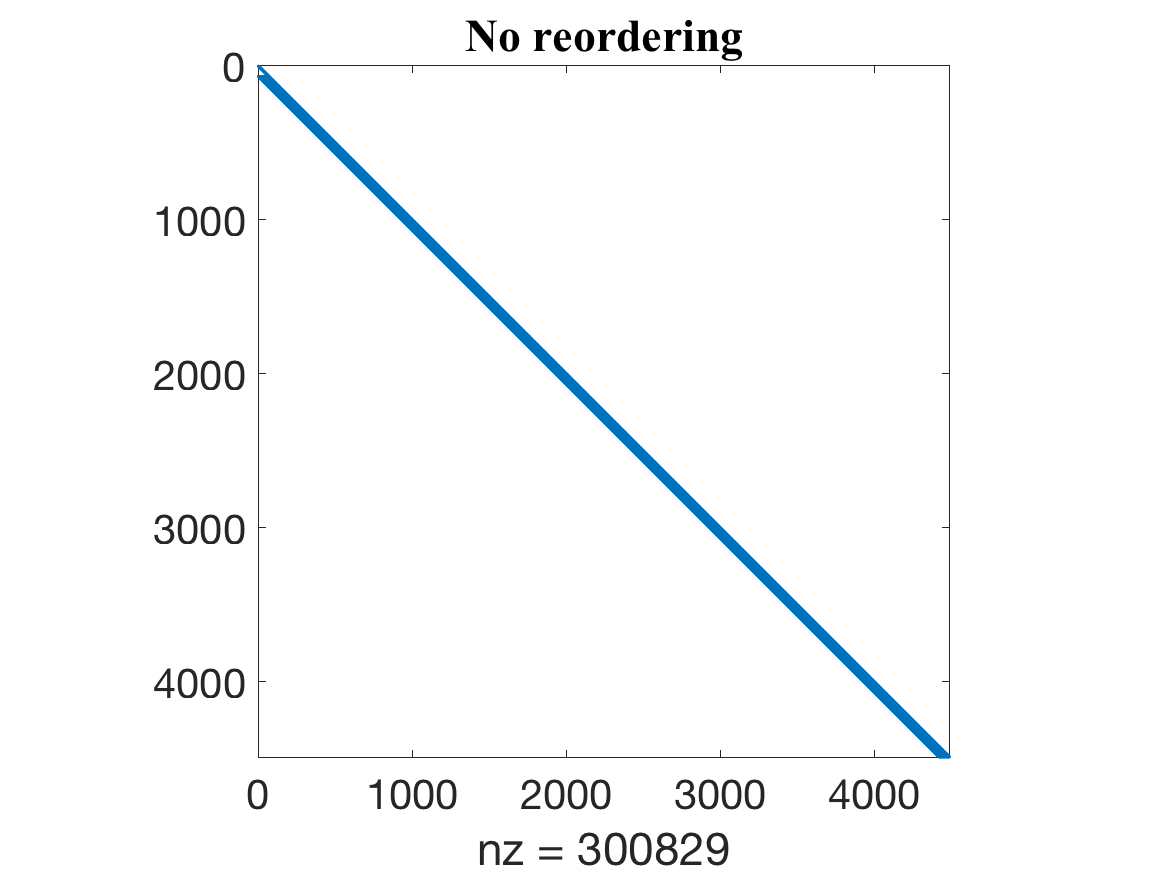
\includegraphics[width=0.45\linewidth]{../Figures/default.png}}\\\hline
  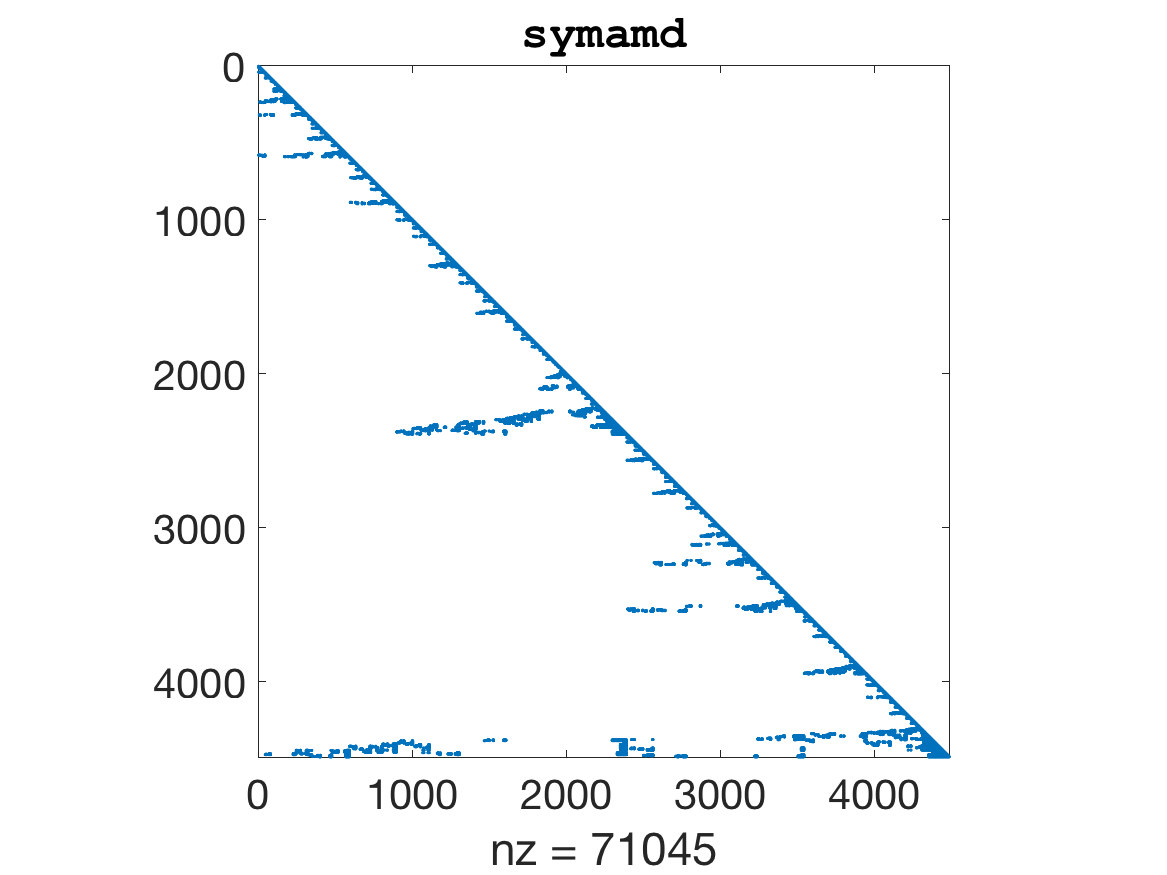
\includegraphics[width=0.45\linewidth]{../Figures/symamd.png}&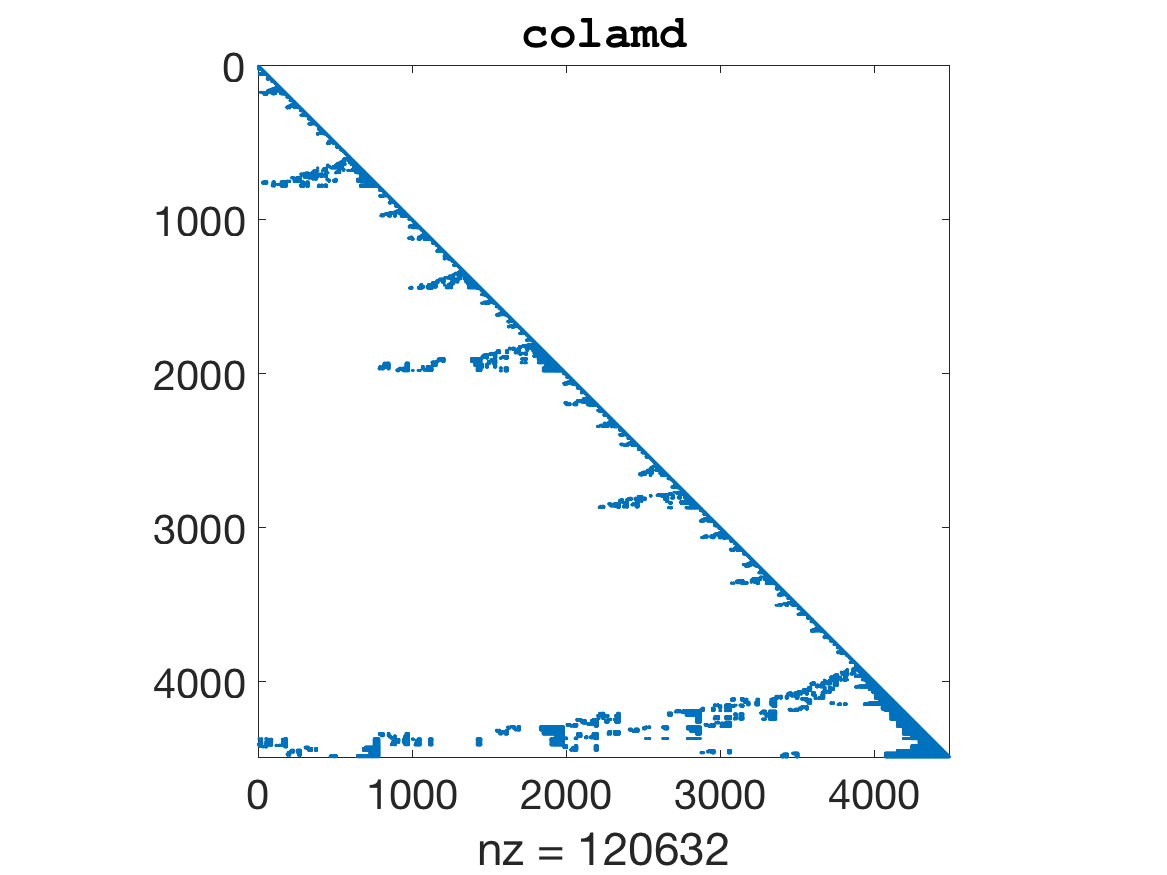
\includegraphics[width=0.45\linewidth]{../Figures/colamd.png}\\\hline
  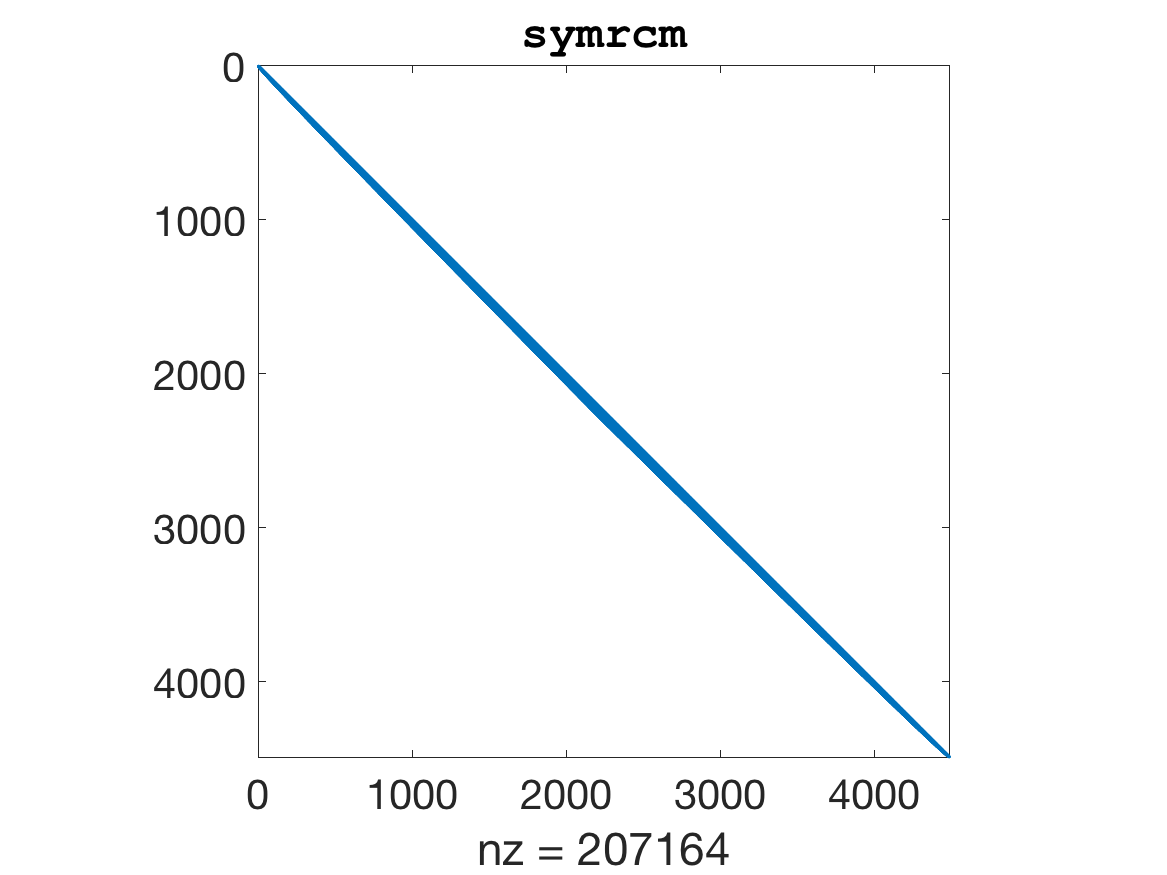
\includegraphics[width=0.45\linewidth]{../Figures/symrcm.png}&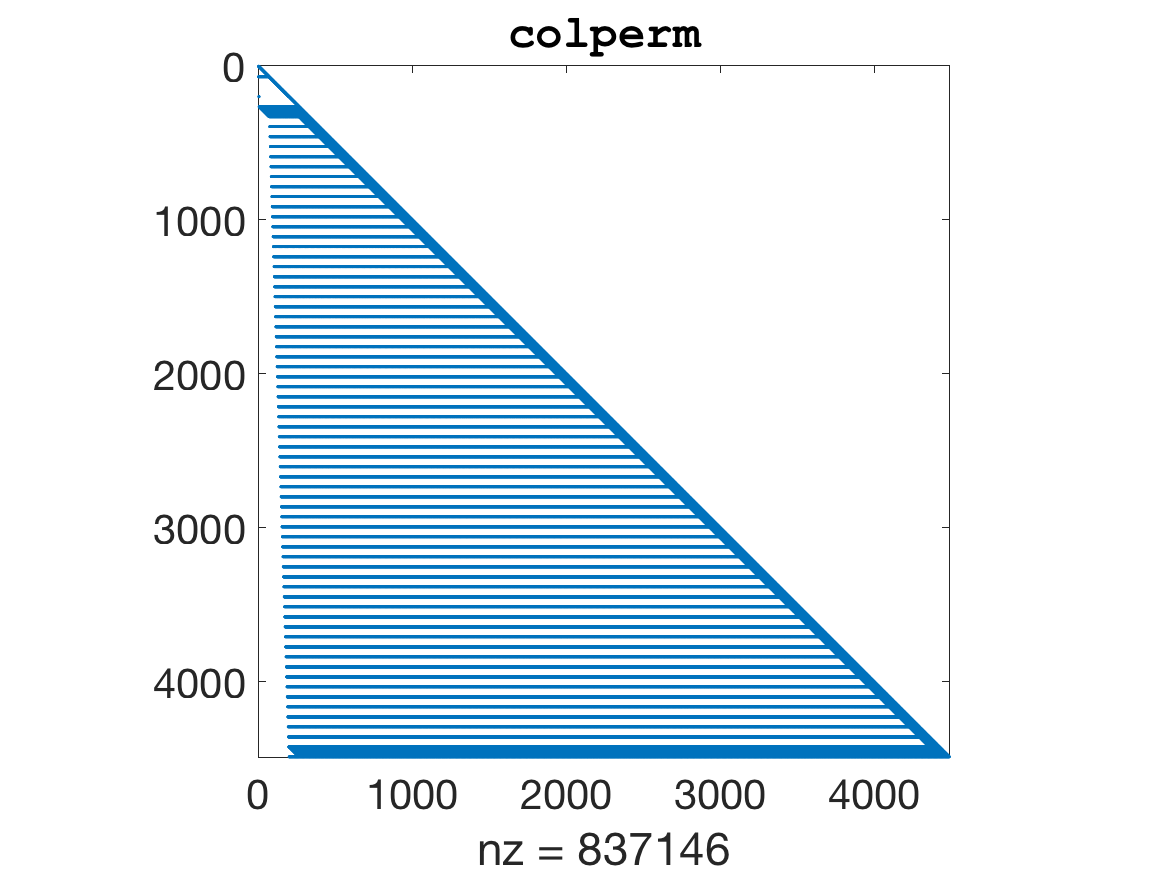
\includegraphics[width=0.45\linewidth]{../Figures/colperm.png}\\\hline
\end{tabular}

Using the following code, my computer ran out of storage after $i=7$.
\lstinputlisting[style=Matlab-editor,basicstyle=\ttfamily\small]{../Code/homework2_1_a_2.m}
\newpage

\newpart
%--------------------------
%    Problem 1 Part B
%--------------------------
\subsection*{(b)}

The following code was used to factor the 3D Laplacian:
\lstinputlisting[style=Matlab-editor,basicstyle=\ttfamily\small]{../Code/homework2_1_b_1.m}
The number of nonzero entries are shown in the following vector:
\begin{equation*}
  \left[
    \begin{array}{c}
      \textrm{No reordering}\\
      \texttt{symamd}\\
      \texttt{colamd}\\
      \texttt{symrcm}\\
      \texttt{colperm}
    \end{array}
  \right]=
  \left[\begin{array}{r}
\texttt{50689}\\
\texttt{15271861}\\
\texttt{36122933}\\
\texttt{38603950}\\
\texttt{222256905}\\
\end{array}
\right].
\end{equation*}
\newpage
The following table shows the output of \texttt{spy(L)}:

\begin{tabular}{|c|c|}
  \hline
  \multicolumn{2}{|c|}{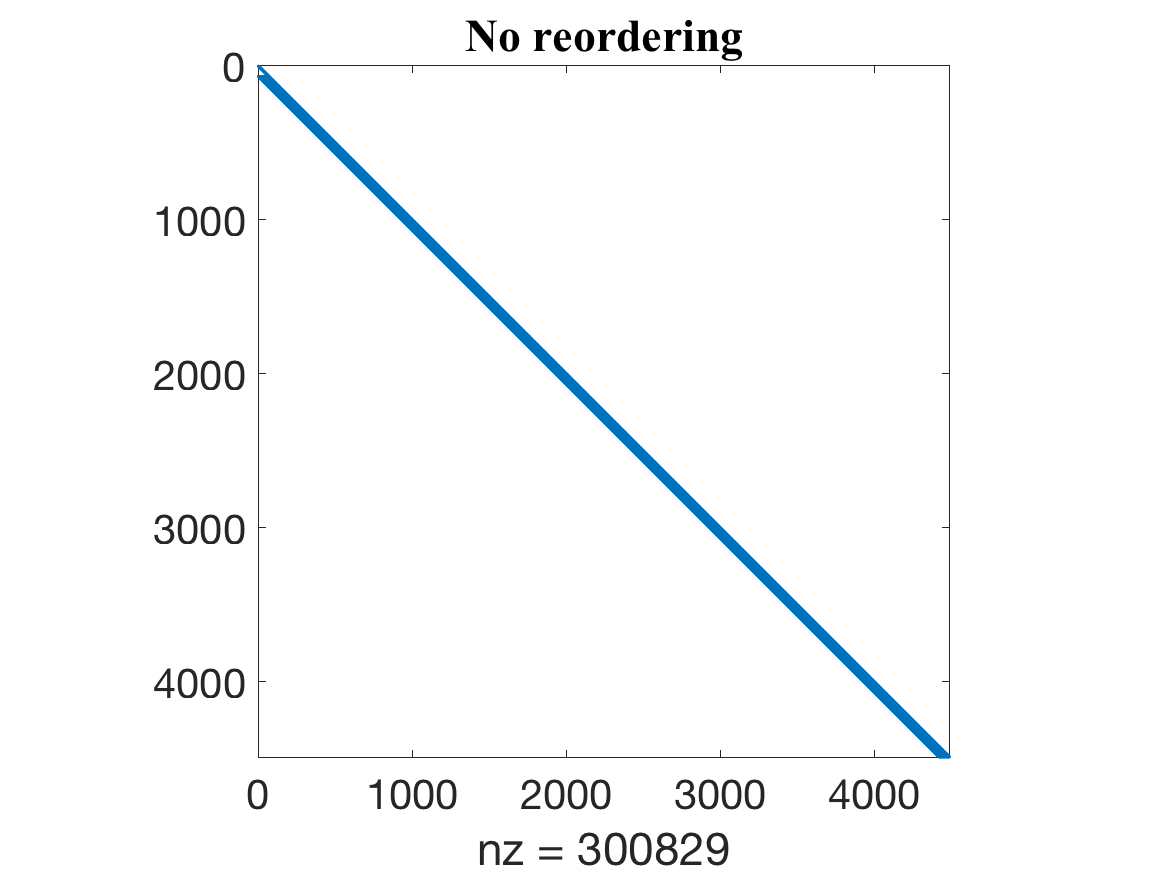
\includegraphics[width=0.45\linewidth]{../Figures/default.png}}\\\hline
  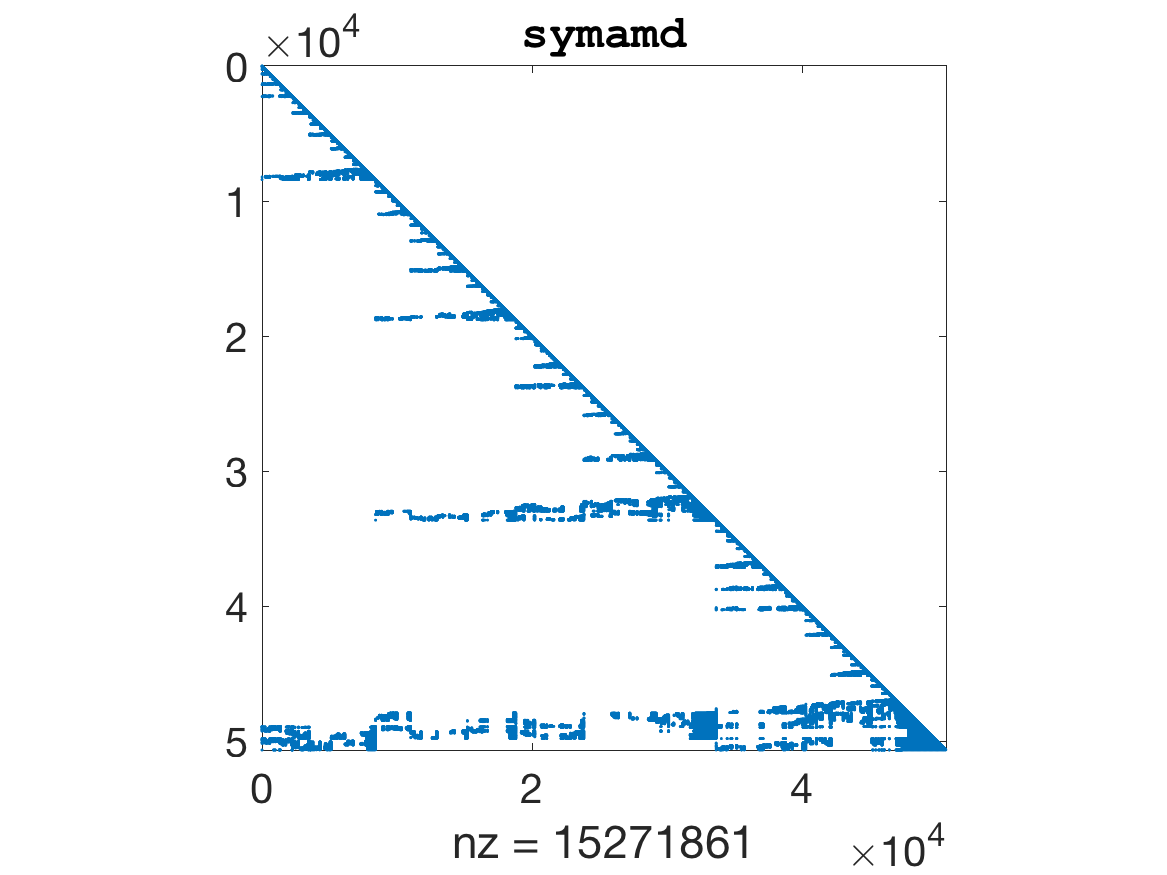
\includegraphics[width=0.45\linewidth]{../Figures/symamdb.png}&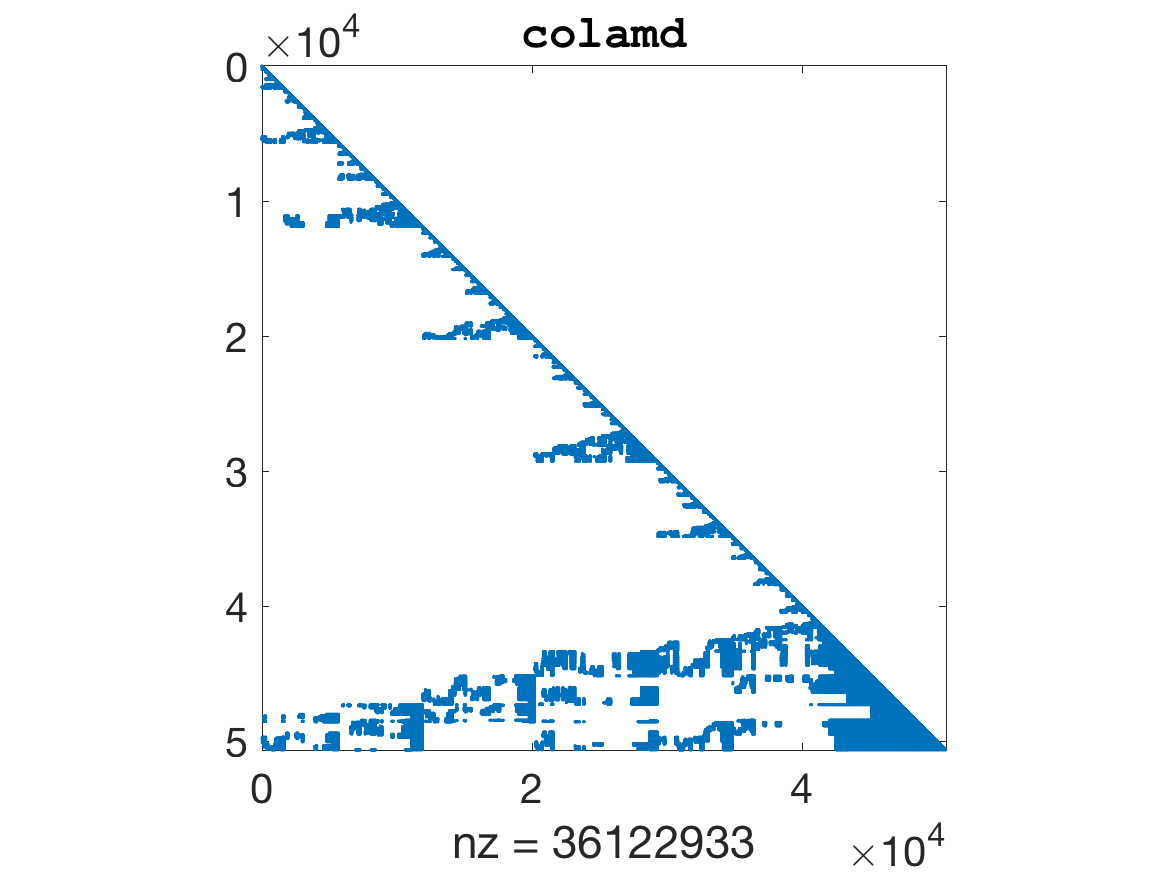
\includegraphics[width=0.45\linewidth]{../Figures/colamdb.png}\\\hline
  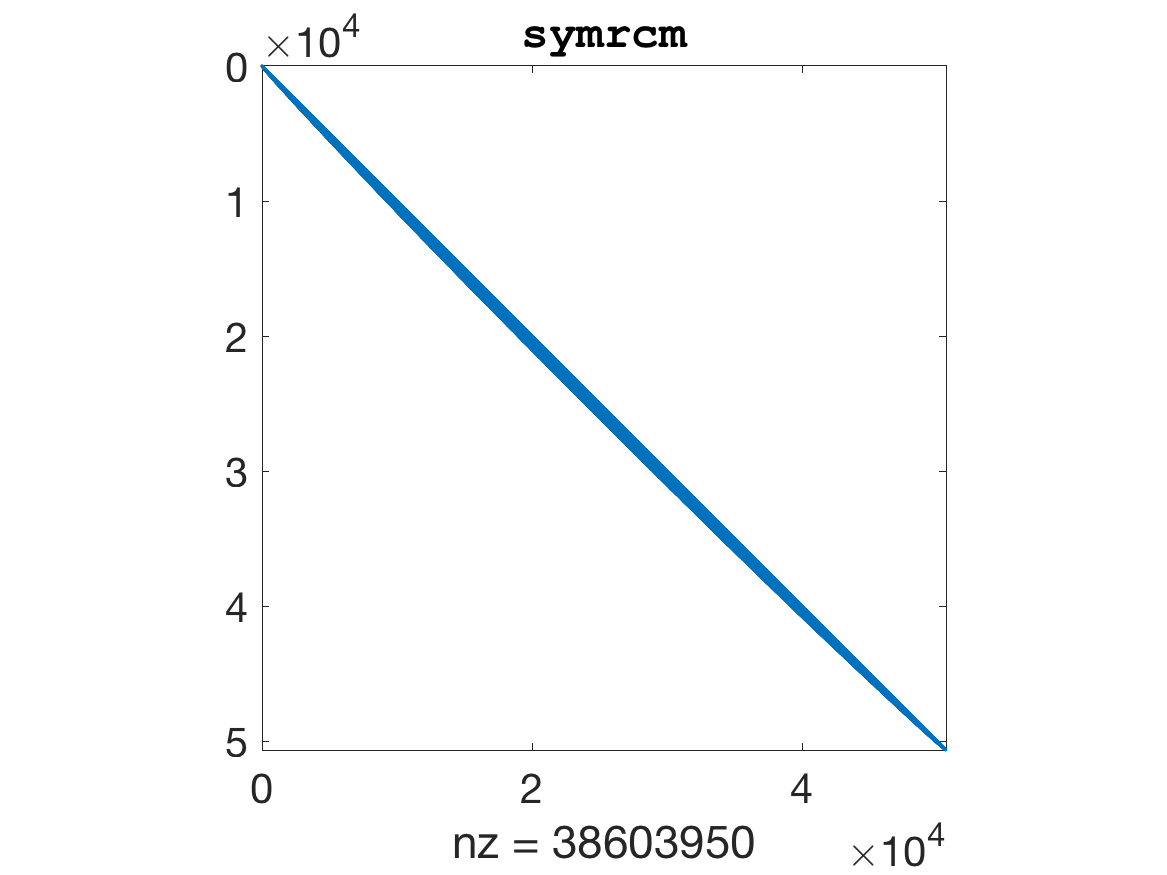
\includegraphics[width=0.45\linewidth]{../Figures/symrcmb.png}&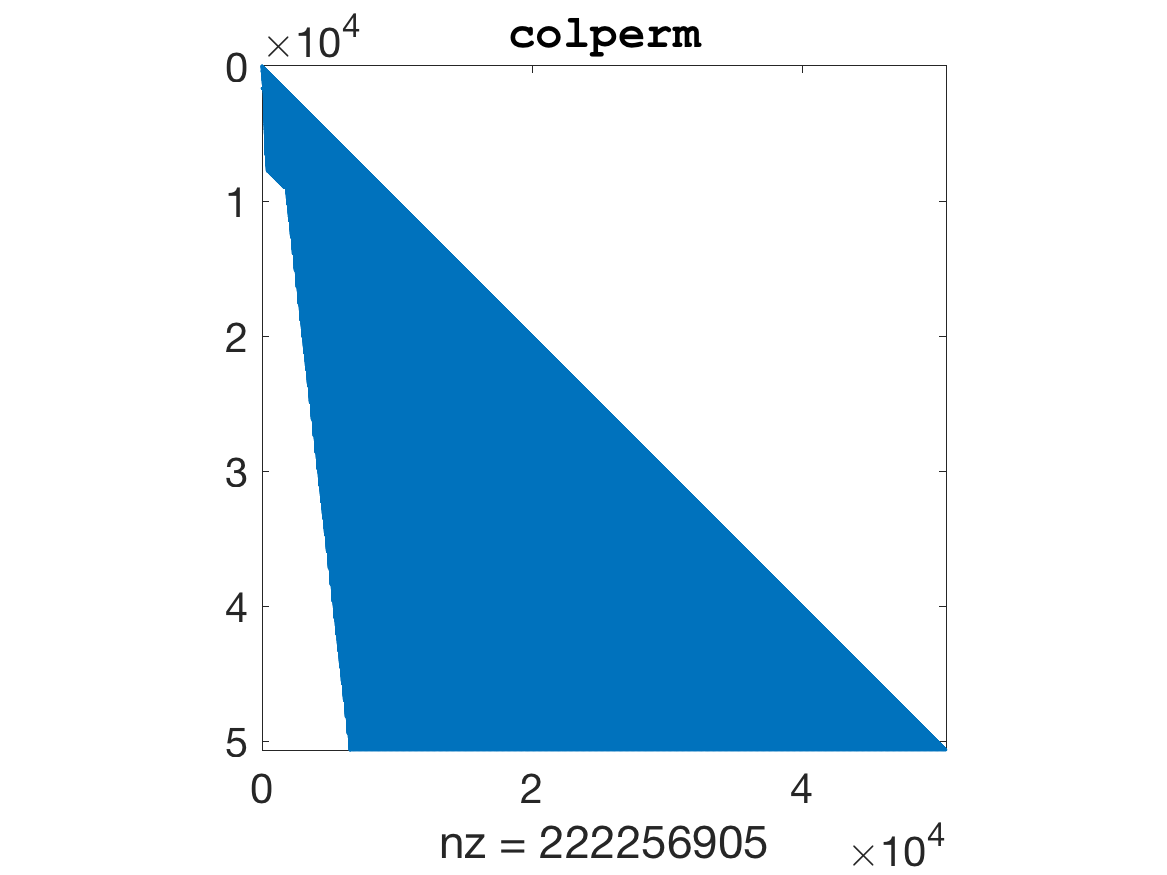
\includegraphics[width=0.45\linewidth]{../Figures/colpermb.png}\\\hline
\end{tabular}

Using the following code, my computer ran out of storage after $i=2$.
\lstinputlisting[style=Matlab-editor,basicstyle=\ttfamily\small]{../Code/homework2_1_b_2.m}
\newpage

\newquestion
%======================================================
%
%                    Problem 2
%
%======================================================
\section*{Problem 2}

\newpart
%--------------------------
%    Problem 2 Part A
%--------------------------
\subsection*{(a)}
\begin{center}
  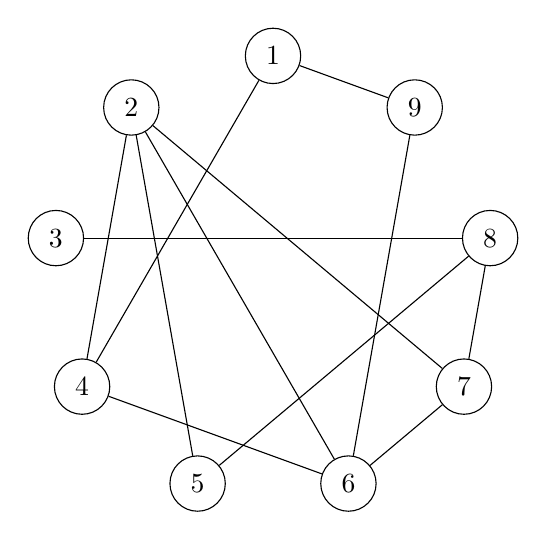
\begin{tikzpicture}
    \tikzset{vertex/.style = {shape=circle,draw,minimum size=2em}}
    \tikzset{edge/.style = {-}}
    
    % vertices
    \foreach \x in {1,...,9}
    {
      \node[vertex] (\x) at ({2.8*cos(90+360*(\x-1)/9)},{2.8*sin(90+360*(\x-1)/9)}) {\x};
      %\draw[edge] (\x) to[in=115+360*\x/9-360/9,out=65+360*\x/9-360/9,loop] (\x);
    }
    
    % edges
    \foreach \y in {4,9} {\draw[edge] (1) to (\y);}
    \foreach \y in {4,5,6,7} {\draw[edge] (2) to (\y);}
    \foreach \y in {8} {\draw[edge] (3) to (\y);}
    \foreach \y in {6} {\draw[edge] (4) to (\y);}
    \foreach \y in {8} {\draw[edge] (5) to (\y);}
    \foreach \y in {7,9} {\draw[edge] (6) to (\y);}
    \foreach \y in {8} {\draw[edge] (7) to (\y);}
    
  \end{tikzpicture}
\end{center}
\newpart
%--------------------------
%    Problem 2 Part B
%--------------------------
\subsection*{(b)}
Since $a_{9,1}\neq0,a_{4,1}\neq0,a_{9,4}=0$, fill-in element at $a_{9,4}$. Thus, the algorithm goes as follows
\begin{tabular}{m{1.2cm}m{3cm}| >{\centering\arraybackslash}l}\hline
  Step 0: & Fill-in step\\
          &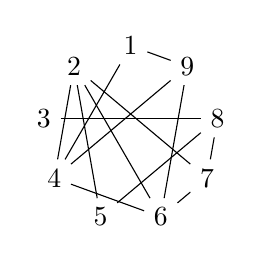
\begin{tikzpicture}[scale=0.4]
            \tikzset{vertex/.style = {}}
            \tikzset{edge/.style = {-}}
            
            % vertices
            \foreach \x in {1,...,9}
            {
              \node[vertex] (\x) at ({2.8*cos(90+360*(\x-1)/9)},{2.8*sin(90+360*(\x-1)/9)}) {\x};
              % \draw[edge] (\x) to[in=115+360*\x/9-360/9,out=65+360*\x/9-360/9,loop] (\x);
            }
            
            % edges
            \foreach \y in {4,9} {\draw[edge] (1) to (\y);}
            \foreach \y in {4,5,6,7} {\draw[edge] (2) to (\y);}
            \foreach \y in {8} {\draw[edge] (3) to (\y);}
            \foreach \y in {6,9} {\draw[edge] (4) to (\y);}
            \foreach \y in {8} {\draw[edge] (5) to (\y);}
            \foreach \y in {7,9} {\draw[edge] (6) to (\y);}
            \foreach \y in {8} {\draw[edge] (7) to (\y);}
            
          \end{tikzpicture}&
                             $d=\left[\begin{array}{ccccccccc}
                                        1/2&1/4&1&1/4&1/2&1/4&1/3&1/3&1/3
                                      \end{array}
                                                                      \right]$\\\hline
  Step 1: & Eliminate node 3. &
                                $p=\left[\begin{array}{ccccccccc}
                                      3
                                    \end{array}
                                \right]$\\
          &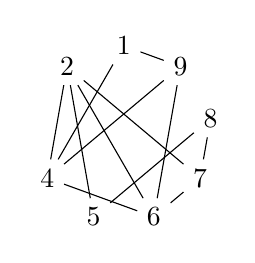
\begin{tikzpicture}[scale=0.4]
            \tikzset{vertex/.style = {}}
            \tikzset{edge/.style = {-}}
            
            % vertices
            \foreach \x in {1,2,4,5,6,7,8,9}
            {
              \node[vertex] (\x) at ({2.8*cos(90+360*(\x-1)/9)},{2.8*sin(90+360*(\x-1)/9)}) {\x};
              % \draw[edge] (\x) to[in=115+360*\x/9-360/9,out=65+360*\x/9-360/9,loop] (\x);
            }
            \foreach \x in {3}
            {
              \node[vertex] (\x) at ({2.8*cos(90+360*(\x-1)/9)},{2.8*sin(90+360*(\x-1)/9)}) {};
            }
            
            % edges
            \foreach \y in {4,9} {\draw[edge] (1) to (\y);}
            \foreach \y in {4,5,6,7} {\draw[edge] (2) to (\y);}
            \foreach \y in {6,9} {\draw[edge] (4) to (\y);}
            \foreach \y in {8} {\draw[edge] (5) to (\y);}
            \foreach \y in {7,9} {\draw[edge] (6) to (\y);}
            \foreach \y in {8} {\draw[edge] (7) to (\y);}
            
          \end{tikzpicture}&
                             $d=\left[\begin{array}{ccccccccc}
                                        1/2&1/4&*&1/4&1/2&1/4&1/3&1/2&1/3
                                      \end{array}
                                                                      \right]$\\\hline
  Step 2: & Eliminate node 1. &
                                $p=\left[\begin{array}{ccccccccc}
                                      3 & 1
                                    \end{array}
                                          \right]$\\
          &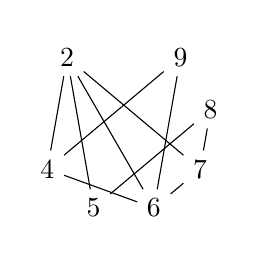
\begin{tikzpicture}[scale=0.4]
            \tikzset{vertex/.style = {}}
            \tikzset{edge/.style = {-}}
            
            % vertices
            \foreach \x in {2,4,5,6,7,8,9}
            {
              \node[vertex] (\x) at ({2.8*cos(90+360*(\x-1)/9)},{2.8*sin(90+360*(\x-1)/9)}) {\x};
              % \draw[edge] (\x) to[in=115+360*\x/9-360/9,out=65+360*\x/9-360/9,loop] (\x);
            }
            \foreach \x in {3,1}
            {
              \node[vertex] (\x) at ({2.8*cos(90+360*(\x-1)/9)},{2.8*sin(90+360*(\x-1)/9)}) {};
            }
            
            % edges
            \foreach \y in {4,5,6,7} {\draw[edge] (2) to (\y);}
            \foreach \y in {6,9} {\draw[edge] (4) to (\y);}
            \foreach \y in {8} {\draw[edge] (5) to (\y);}
            \foreach \y in {7,9} {\draw[edge] (6) to (\y);}
            \foreach \y in {8} {\draw[edge] (7) to (\y);}
            
          \end{tikzpicture}&
                             $d=\left[\begin{array}{ccccccccc}
                                        *&1/4&*&1/3&1/2&1/4&1/3&1/2&1/2
                                      \end{array}
                                                                    \right]$\\
\end{tabular}\newpage
\begin{tabular}{m{1.2cm}m{3cm}| >{\centering\arraybackslash}l}\hline
  Step 3: & Eliminate node 5. &
                                $p=\left[\begin{array}{ccccccccc}
                                           3 & 1 & 5
                                         \end{array}
                                                   \right]$\\
          &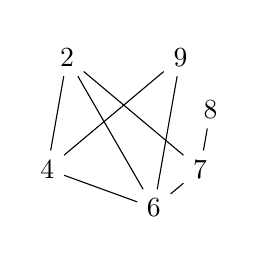
\begin{tikzpicture}[scale=0.4]
            \tikzset{vertex/.style = {}}
            \tikzset{edge/.style = {-}}
            
            % vertices
            \foreach \x in {2,4,6,7,8,9}
            {
              \node[vertex] (\x) at ({2.8*cos(90+360*(\x-1)/9)},{2.8*sin(90+360*(\x-1)/9)}) {\x};
              % \draw[edge] (\x) to[in=115+360*\x/9-360/9,out=65+360*\x/9-360/9,loop] (\x);
            }
            \foreach \x in {3,1,5}
            {
              \node[vertex] (\x) at ({2.8*cos(90+360*(\x-1)/9)},{2.8*sin(90+360*(\x-1)/9)}) {};
            }
            
            % edges
            \foreach \y in {4,6,7} {\draw[edge] (2) to (\y);}
            \foreach \y in {6,9} {\draw[edge] (4) to (\y);}
            \foreach \y in {7,9} {\draw[edge] (6) to (\y);}
            \foreach \y in {8} {\draw[edge] (7) to (\y);}
            
          \end{tikzpicture}&
                             $d=\left[\begin{array}{ccccccccc}
                                        *&1/3&*&1/3&*&1/4&1/3&1&1/2
                                      \end{array}
                                                                 \right]$\\\hline
  Step 4: & Eliminate node 8. &
                                $p=\left[\begin{array}{ccccccccc}
                                           3 & 1 & 5 & 8
                                         \end{array}
                                                       \right]$\\
          &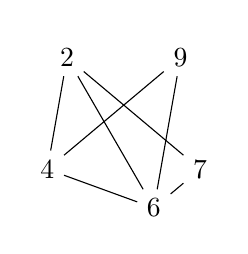
\begin{tikzpicture}[scale=0.4]
            \tikzset{vertex/.style = {}}
            \tikzset{edge/.style = {-}}
            
            % vertices
            \foreach \x in {2,4,6,7,9}
            {
              \node[vertex] (\x) at ({2.8*cos(90+360*(\x-1)/9)},{2.8*sin(90+360*(\x-1)/9)}) {\x};
              % \draw[edge] (\x) to[in=115+360*\x/9-360/9,out=65+360*\x/9-360/9,loop] (\x);
            }
            \foreach \x in {3,1,5,8}
            {
              \node[vertex] (\x) at ({2.8*cos(90+360*(\x-1)/9)},{2.8*sin(90+360*(\x-1)/9)}) {};
            }
            
            % edges
            \foreach \y in {4,6,7} {\draw[edge] (2) to (\y);}
            \foreach \y in {6,9} {\draw[edge] (4) to (\y);}
            \foreach \y in {7,9} {\draw[edge] (6) to (\y);}
            
          \end{tikzpicture}&
                             $d=\left[\begin{array}{ccccccccc}
                                        *&1/3&*&1/3&*&1/4&1/2&*&1/2
                                      \end{array}
                                                                 \right]$\\\hline
  Step 5: & Eliminate node 7. &
                                $p=\left[\begin{array}{ccccccccc}
                                           3 & 1 & 5 & 8 & 7
                                         \end{array}
                                                           \right]$\\
          &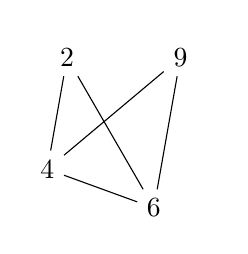
\begin{tikzpicture}[scale=0.4]
            \tikzset{vertex/.style = {}}
            \tikzset{edge/.style = {-}}
            
            % vertices
            \foreach \x in {2,4,6,9}
            {
              \node[vertex] (\x) at ({2.8*cos(90+360*(\x-1)/9)},{2.8*sin(90+360*(\x-1)/9)}) {\x};
              % \draw[edge] (\x) to[in=115+360*\x/9-360/9,out=65+360*\x/9-360/9,loop] (\x);
            }
            \foreach \x in {3,1,5,8,7}
            {
              \node[vertex] (\x) at ({2.8*cos(90+360*(\x-1)/9)},{2.8*sin(90+360*(\x-1)/9)}) {};
            }
            
            % edges
            \foreach \y in {4,6} {\draw[edge] (2) to (\y);}
            \foreach \y in {6,9} {\draw[edge] (4) to (\y);}
            \foreach \y in {9} {\draw[edge] (6) to (\y);}
            
          \end{tikzpicture}&
                             $d=\left[\begin{array}{ccccccccc}
                                        *&1/2&*&1/3&*&1/3&*&*&1/2
                                      \end{array}
                                                               \right]$\\\hline
  Step 6: & Eliminate node 2. &
                                $p=\left[\begin{array}{ccccccccc}
                                           3 & 1 & 5 & 8 & 7 & 2
                                         \end{array}
                                                           \right]$\\
          &\begin{tikzpicture}[scale=0.4]
            \tikzset{vertex/.style = {}}
            \tikzset{edge/.style = {-}}
            
            % vertices
            \foreach \x in {4,6,9}
            {
              \node[vertex] (\x) at ({2.8*cos(90+360*(\x-1)/9)},{2.8*sin(90+360*(\x-1)/9)}) {\x};
              % \draw[edge] (\x) to[in=115+360*\x/9-360/9,out=65+360*\x/9-360/9,loop] (\x);
            }
            \foreach \x in {3,1,5,8,7,2}
            {
              \node[vertex] (\x) at ({2.8*cos(90+360*(\x-1)/9)},{2.8*sin(90+360*(\x-1)/9)}) {};
            }
            
            % edges
            \foreach \y in {6,9} {\draw[edge] (4) to (\y);}
            \foreach \y in {9} {\draw[edge] (6) to (\y);}
            
          \end{tikzpicture}&
                             $d=\left[\begin{array}{ccccccccc}
                                        *&*&*&1/2&*&1/2&*&*&1/2
                                      \end{array}
                                                             \right]$\\\hline
  Step 7: & Eliminate node 4. &
                                $p=\left[\begin{array}{ccccccccc}
                                           3 & 1 & 5 & 8 & 7 & 2 & 4
                                         \end{array}
                                                           \right]$\\
          &\begin{tikzpicture}[scale=0.4]
            \tikzset{vertex/.style = {}}
            \tikzset{edge/.style = {-}}
            
            % vertices
            \foreach \x in {6,9}
            {
              \node[vertex] (\x) at ({2.8*cos(90+360*(\x-1)/9)},{2.8*sin(90+360*(\x-1)/9)}) {\x};
              % \draw[edge] (\x) to[in=115+360*\x/9-360/9,out=65+360*\x/9-360/9,loop] (\x);
            }
            \foreach \x in {3,1,5,8,7,2,4}
            {
              \node[vertex] (\x) at ({2.8*cos(90+360*(\x-1)/9)},{2.8*sin(90+360*(\x-1)/9)}) {};
            }
            
            % edges
            \foreach \y in {9} {\draw[edge] (6) to (\y);}
            
          \end{tikzpicture}&
                             $d=\left[\begin{array}{ccccccccc}
                                        *&*&*&*&*&1&*&*&1
                                      \end{array}
                                                         \right]$\\\hline
  Step 8: & Eliminate node 6. &
                                $p=\left[\begin{array}{ccccccccc}
                                           3 & 1 & 5 & 8 & 7 & 2 & 4 & 6
                                         \end{array}
                                                           \right]$\\
          &\\\hline
  Final: & Eliminate node 9. &
                               $p=\left[\begin{array}{ccccccccc}
                                          3 & 1 & 5 & 8 & 7 & 2 & 4 & 6 & 9
                                        \end{array}
                                                                          \right]$\\
\end{tabular}\newpage

\newpart
%--------------------------
%    Problem 2 Part C
%--------------------------
\subsection*{(c)}
\begin{equation*}
  A=\left[
    \begin{array}{ccccccccc}
      *&0&0&*&0&0&0&0&0\\
      0&*&0&0&0&0&*&0&*\\
      0&0&*&*&0&*&0&0&0\\
      *&0&*&*&*&0&0&0&0\\
      0&0&0&*&*&*&0&*&0\\
      0&0&*&0&*&*&*&*&0\\
      0&*&0&0&0&*&*&*&0\\
      0&0&0&0&*&*&*&*&*\\
      0&*&0&0&0&0&0&*&*
    \end{array}\right]
\end{equation*}

\newquestion
%======================================================
%
%                    Problem 3
%
%======================================================
\section*{Problem 3}

\newpart
%--------------------------
%    Problem 3 Part A
%--------------------------
\subsection*{(a)}
There would be 17 fill-in elements in positions $u_{2,1}$, $u_{2,2}$, $u_{2,4}$, $u_{4,1}$, $u_{4,2}$, $u_{4,4}$, $u_{5,1}$, $u_{5,2}$, $u_{5,4}$, $u_{7,1}$, $u_{7,4}$, $u_{10,1}$, $u_{10,2}$, $u_{10,4}$, $u_{11,1}$, $u_{11,2}$, $u_{11,4}$.

\newpart
%--------------------------
%    Problem 3 Part B
%--------------------------
\subsection*{(b)}
There would be a pivot at $u_{2,11}$. After the pivot,
\begin{equation*}
  U^{(k)}=\left[
    \begin{array}{ccccccccccc}
      *&0&0&0&0&0&0&0&0&0&*\\
      0&*&*&0&*&0&0&0&0&0&*\\
      0&0&0&*&*&0&0&0&*&*&0\\
      0&0&0&0&0&*&0&0&*&0&*\\
      0&0&0&0&0&0&*&*&0&0&*\\
      *&0&0&*&0&0&0&0&0&*&0\\
      0&0&*&*&0&*&0&0&0&*&*\\
      0&*&0&0&0&*&0&0&0&*&0\\
      0&0&0&0&0&0&*&*&0&*&0\\
      0&0&0&*&0&0&0&*&0&0&*\\
      *&0&0&0&0&*&0&0&0&0&*
    \end{array}\right],
\end{equation*}
so there would only be one pivot at $u_{5,11}$.

\newquestion
%======================================================
%
%                    Problem 4
%
%======================================================
\section*{Problem 4}

\newpart
%--------------------------
%    Problem 4 Part A
%--------------------------
\subsection*{(a)}
The following function was used to find the $J$,$I$, and $V_L$ matrix for the compressed sparse column format for a lower-triangular matrix
\lstinputlisting[style=Matlab-editor,basicstyle=\ttfamily\small]{../Code/comp_l_tri.m}
The following code was used on the \texttt{small\_ex.mat} example
\lstinputlisting[style=Matlab-editor,basicstyle=\ttfamily\small]{../Code/homework2_4_a_1.m}
and the following code was used for the \texttt{large\_ex.mat} example
\lstinputlisting[style=Matlab-editor,basicstyle=\ttfamily\small]{../Code/homework2_4_a_2.m}
The output for the \texttt{small\_ex.mat} example is
\begin{equation*}
  J=\left[\begin{array}{r}
\texttt{1}\\
\texttt{3}\\
\texttt{4}\\
\texttt{9}\\
\texttt{2}\\
\texttt{4}\\
\texttt{5}\\
\texttt{8}\\
\texttt{9}\\
\texttt{3}\\
\texttt{5}\\
\texttt{7}\\
\texttt{8}\\
\texttt{4}\\
\texttt{6}\\
\texttt{7}\\
\texttt{8}\\
\texttt{9}\\
\texttt{5}\\
\texttt{8}\\
\texttt{9}\\
\texttt{6}\\
\texttt{7}\\
\texttt{8}\\
\texttt{9}\\
\texttt{7}\\
\texttt{8}\\
\texttt{8}\\
\texttt{10}\\
\texttt{9}\\
\texttt{10}\\
\end{array}
\right],\quad I=\left[\begin{array}{r}
\texttt{1}\\
\texttt{5}\\
\texttt{10}\\
\texttt{14}\\
\texttt{19}\\
\texttt{22}\\
\texttt{26}\\
\texttt{28}\\
\texttt{30}\\
\texttt{31}\\
\texttt{32}\\
\end{array}
\right],\quad V_L=\left[\begin{array}{r}
\texttt{1.000000000000000e+00}\\
\texttt{8.127286465304295e-01}\\
\texttt{2.578478773046358e-01}\\
\texttt{-7.969322223753756e-01}\\
\texttt{1.000000000000000e+00}\\
\texttt{-8.907667695526849e-01}\\
\texttt{2.565826406430549e-03}\\
\texttt{-1.365576562315056e-01}\\
\texttt{9.951206990243782e-01}\\
\texttt{1.000000000000000e+00}\\
\texttt{-2.869666020396466e-02}\\
\texttt{7.888955111347864e-01}\\
\texttt{-7.249068104658705e-01}\\
\texttt{1.000000000000000e+00}\\
\texttt{8.547124499962497e-01}\\
\texttt{8.349876648322339e-01}\\
\texttt{4.271480231886315e-01}\\
\texttt{2.366747672438800e-01}\\
\texttt{1.000000000000000e+00}\\
\texttt{8.720546533795395e-01}\\
\texttt{-7.504519186790148e-01}\\
\texttt{1.000000000000000e+00}\\
\texttt{2.929548648516276e-01}\\
\texttt{6.663039713385901e-01}\\
\texttt{-2.034355435624491e-01}\\
\texttt{1.000000000000000e+00}\\
\texttt{6.704410209562610e-01}\\
\texttt{1.000000000000000e+00}\\
\texttt{1.045232337167099e-01}\\
\texttt{1.000000000000000e+00}\\
\texttt{1.000000000000000e+00}\\
\end{array}
\right]
\end{equation*}
and \texttt{large\_ex.mat} example is
\begin{equation*}
  \left[
    \begin{array}{r}
      I(50000)\\
      I(100000)\\
      I(150000)\\
      I(200000)\\
      I(250000)
    \end{array}
  \right]=\left[\begin{array}{r}
\texttt{376955}\\
\texttt{1762353}\\
\texttt{4716326}\\
\texttt{12466445}\\
\texttt{15513326}\\
\end{array}
\right].
\end{equation*}

\newpage
\newpart
%--------------------------
%    Problem 4 Part B
%--------------------------
\subsection*{(b)}

The following function was used to find the $J$,$I$, and $V_L$ matrix for the compressed sparse column format for an upper-triangular matrix
\lstinputlisting[style=Matlab-editor,basicstyle=\ttfamily\small]{../Code/comp_u_tri.m}
The following code was used on the \texttt{small\_ex.mat} example
\lstinputlisting[style=Matlab-editor,basicstyle=\ttfamily\small]{../Code/homework2_4_b_1.m}
and the following code was used for the \texttt{large\_ex.mat} example
\lstinputlisting[style=Matlab-editor,basicstyle=\ttfamily\small]{../Code/homework2_4_b_2.m}
The output for the \texttt{small\_ex.mat} example is
\begin{equation*}
  J=\left[\begin{array}{r}
\texttt{1}\\
\texttt{2}\\
\texttt{1}\\
\texttt{3}\\
\texttt{1}\\
\texttt{2}\\
\texttt{4}\\
\texttt{2}\\
\texttt{3}\\
\texttt{5}\\
\texttt{4}\\
\texttt{6}\\
\texttt{3}\\
\texttt{4}\\
\texttt{6}\\
\texttt{7}\\
\texttt{2}\\
\texttt{3}\\
\texttt{4}\\
\texttt{5}\\
\texttt{6}\\
\texttt{7}\\
\texttt{8}\\
\texttt{1}\\
\texttt{2}\\
\texttt{4}\\
\texttt{5}\\
\texttt{6}\\
\texttt{9}\\
\texttt{8}\\
\texttt{10}\\
\end{array}
\right],\quad I=\left[\begin{array}{r}
\texttt{1}\\
\texttt{2}\\
\texttt{4}\\
\texttt{7}\\
\texttt{10}\\
\texttt{12}\\
\texttt{16}\\
\texttt{23}\\
\texttt{29}\\
\texttt{31}\\
\texttt{32}\\
\end{array}
\right],\quad V_L=\left[\begin{array}{r}
\texttt{-7.227965685152800e-01}\\
\texttt{1.764187707789873e-01}\\
\texttt{-2.676863990901244e-01}\\
\texttt{6.135190893222113e-01}\\
\texttt{7.561571552311852e-03}\\
\texttt{-2.081132255329154e-02}\\
\texttt{7.540974467700878e-01}\\
\texttt{-2.937163741220890e-01}\\
\texttt{-1.011128868565034e-01}\\
\texttt{9.270605736868538e-01}\\
\texttt{-9.154044041709144e-01}\\
\texttt{9.459166682812694e-01}\\
\texttt{-6.215863137552480e-01}\\
\texttt{3.342406000801499e-01}\\
\texttt{1.728792293578358e-01}\\
\texttt{3.502248328102306e-01}\\
\texttt{-2.779559016106783e-01}\\
\texttt{2.405568541421710e-01}\\
\texttt{6.223017702005704e-01}\\
\texttt{-9.614850451717172e-01}\\
\texttt{-8.322529834342003e-01}\\
\texttt{9.496033343697807e-01}\\
\texttt{3.026990648307066e-01}\\
\texttt{-5.375243676712955e-01}\\
\texttt{-1.930177137508202e-01}\\
\texttt{-7.559589634957409e-01}\\
\texttt{-4.631223572054337e-01}\\
\texttt{-4.843076597747906e-01}\\
\texttt{-3.366695225147414e-01}\\
\texttt{-6.955319742741071e-01}\\
\texttt{-3.039846805677731e-01}\\
\end{array}
\right]
\end{equation*}
and \texttt{large\_ex.mat} example is
\begin{equation*}
  \left[
    \begin{array}{r}
      I(50000)\\
      I(100000)\\
      I(150000)\\
      I(200000)\\
      I(250000)
    \end{array}
  \right]=\left[\begin{array}{r}
\texttt{209895}\\
\texttt{1442487}\\
\texttt{4084327}\\
\texttt{14906857}\\
\texttt{17772355}\\
\end{array}
\right].
\end{equation*}

\newpage
\newpart
%--------------------------
%    Problem 4 Part C
%--------------------------
\subsection*{(c)}
The following functions were written to solve the equations $Lc=b$ and $Ux=c$ respectively
\lstinputlisting[style=Matlab-editor,basicstyle=\ttfamily\small]{../Code/solve_l.m}
\lstinputlisting[style=Matlab-editor,basicstyle=\ttfamily\small]{../Code/solve_u.m}
The following code was used on the \texttt{small\_ex.mat} example
\lstinputlisting[style=Matlab-editor,basicstyle=\ttfamily\small]{../Code/homework2_4_c_1.m}
and the following code was used for the \texttt{large\_ex.mat} example
\lstinputlisting[style=Matlab-editor,basicstyle=\ttfamily\small]{../Code/homework2_4_c_2.m}
The output for the \texttt{small\_ex.mat} example is
\begin{equation*}
  x=\left[\begin{array}{r}
\texttt{-7.368997733798020e+00}\\
\texttt{-3.412065799871883e+01}\\
\texttt{2.493451030044967e+01}\\
\texttt{-2.682899840821154e+01}\\
\texttt{-9.180874775319783e+00}\\
\texttt{-1.237568442840570e+01}\\
\texttt{2.593887743663491e+01}\\
\texttt{-6.717855384133224e+00}\\
\texttt{-4.296837993924318e+00}\\
\texttt{-1.097654778394844e+00}\\
\end{array}
\right]
\end{equation*}
and \texttt{large\_ex.mat} example is
\begin{equation*}
  \left[
    \begin{array}{r}
      x(50000)\\
      x(100000)\\
      x(150000)\\
      x(200000)\\
      x(250000)
    \end{array}
  \right]=\left[\begin{array}{r}
\texttt{-7.306985715493668e+04}\\
\texttt{-5.686028360745258e+05}\\
\texttt{5.850981452463222e+04}\\
\texttt{-6.238599598901578e+04}\\
\texttt{4.381939017807725e+06}\\
\end{array}
\right].
\end{equation*}

\newquestion
%======================================================
%
%                    Problem 5
%
%======================================================
\section*{Problem 5}
The following code was used.
\lstinputlisting[style=Matlab-editor,basicstyle=\ttfamily\small]{../Code/homework2_5_1.m}\newpage

The output for \texttt{large\_ex1.mat}

\newpart
%--------------------------
%    Problem 5 Part i
%--------------------------
\subsection*{Ex. 1: (i)}
\hspace{6cm}Without scaling\hspace{3.25cm}With scaling
\begin{equation*}
    \left.\begin{array}{c}
      \texttt{nnz}(L)\\
      \texttt{nnz}(U)\\
      ||b-Ax||_2/||b||_2\\
      x(1)\\
      x(30000)\\
      x(70000)\\
      x(140000)\\
      x(200002)
    \end{array}\right|\quad
    \left.\begin{array}{r}
\texttt{4.816814200000000e+07}\\
\texttt{7.515763800000000e+07}\\
\texttt{2.828029206810877e-12}\\
\texttt{3.724469259680818e-01}\\
\texttt{-9.486769919656040e-01}\\
\texttt{5.609874735302742e-02}\\
\texttt{5.158011280782167e-02}\\
\texttt{3.492542265989640e-02}\\
\end{array}
\right|\qquad
    \begin{array}{r}
\texttt{2.607293400000000e+07}\\
\texttt{4.119203700000000e+07}\\
\texttt{6.790398425331222e-14}\\
\texttt{3.724469259680818e-01}\\
\texttt{-9.486769948691244e-01}\\
\texttt{5.609874645819704e-02}\\
\texttt{5.158011140559619e-02}\\
\texttt{3.492542265861234e-02}\\
\end{array}
.
\end{equation*}

\newpart
%--------------------------
%    Problem 5 Part ii
%--------------------------
\subsection*{Ex. 1: (ii)}
\hspace{6cm}Without scaling\hspace{3.25cm}With scaling
\begin{equation*}
    \left.\begin{array}{c}
      \texttt{nnz}(L)\\
      \texttt{nnz}(U)\\
      ||b-Ax||_2/||b||_2\\
      x(1)\\
      x(30000)\\
      x(70000)\\
      x(140000)\\
      x(200002)
    \end{array}\right|\quad
    \left.\begin{array}{r}
\texttt{4.810847900000000e+07}\\
\texttt{1.027379140000000e+08}\\
\texttt{1.067252484791601e-11}\\
\texttt{3.724469259680818e-01}\\
\texttt{-9.486769975350847e-01}\\
\texttt{5.609874791210737e-02}\\
\texttt{5.158011150167822e-02}\\
\texttt{3.492542265822163e-02}\\
\end{array}
\right|\qquad
    \begin{array}{r}
\texttt{2.308868800000000e+07}\\
\texttt{3.763303400000000e+07}\\
\texttt{8.116366886591767e-14}\\
\texttt{3.724469259680818e-01}\\
\texttt{-9.486769973752108e-01}\\
\texttt{5.609874620224603e-02}\\
\texttt{5.158011103064770e-02}\\
\texttt{3.492542265822110e-02}\\
\end{array}
.
\end{equation*}

\newpart
%--------------------------
%    Problem 5 Part iii
%--------------------------
\subsection*{Ex. 1: (iii)}
\hspace{6cm}Without scaling\hspace{3.25cm}With scaling
\begin{equation*}
    \left.\begin{array}{c}
      \texttt{nnz}(L)\\
      \texttt{nnz}(U)\\
      ||b-Ax||_2/||b||_2\\
      x(1)\\
      x(30000)\\
      x(70000)\\
      x(140000)\\
      x(200002)
    \end{array}\right|\quad
    \left.\begin{array}{r}
\texttt{4.129774200000000e+07}\\
\texttt{8.125790400000000e+07}\\
\texttt{2.374530280936845e-14}\\
\texttt{3.724469259680818e-01}\\
\texttt{-9.486769978902629e-01}\\
\texttt{5.609874623542198e-02}\\
\texttt{5.158011102075557e-02}\\
\texttt{3.492542265976455e-02}\\
\end{array}
\right|\qquad
    \begin{array}{r}
\texttt{2.296480200000000e+07}\\
\texttt{3.368607300000000e+07}\\
\texttt{5.125021168696811e-14}\\
\texttt{3.724469259680818e-01}\\
\texttt{-9.486769983414199e-01}\\
\texttt{5.609874579025122e-02}\\
\texttt{5.158011071012165e-02}\\
\texttt{3.492542265839199e-02}\\
\end{array}
.
\end{equation*}\newpage

The output for \texttt{large\_ex2.mat}

\newpart
%--------------------------
%    Problem 5 Part i
%--------------------------
\subsection*{Ex. 2: (i)}
\hspace{6cm}Without scaling\hspace{3.25cm}With scaling
\begin{equation*}
    \left.\begin{array}{c}
      \texttt{nnz}(L)\\
      \texttt{nnz}(U)\\
      ||b-Ax||_2/||b||_2\\
      x(1)\\
      x(30000)\\
      x(70000)\\
      x(140000)\\
      x(200002)
    \end{array}\right|\quad
    \left.\begin{array}{r}
\texttt{3.188442500000000e+07}\\
\texttt{4.444986200000000e+07}\\
\texttt{1.650718270551992e-16}\\
\texttt{-5.870862540210242e-01}\\
\texttt{-9.401644284862181e-01}\\
\texttt{6.591485582451860e-02}\\
\texttt{8.626100798318471e-01}\\
\texttt{-2.718282595836798e-02}\\
\end{array}
\right|\qquad
    \begin{array}{r}
\texttt{3.033252700000000e+07}\\
\texttt{4.354803300000000e+07}\\
\texttt{2.582444141156649e-14}\\
\texttt{-5.870862540907285e-01}\\
\texttt{-9.401644284864308e-01}\\
\texttt{6.591485582454848e-02}\\
\texttt{8.626097937227244e-01}\\
\texttt{-2.718282681590964e-02}\\
\end{array}
.
\end{equation*}

\newpart
%--------------------------
%    Problem 5 Part ii
%--------------------------
\subsection*{Ex. 2: (ii)}
\hspace{6cm}Without scaling\hspace{3.25cm}With scaling
\begin{equation*}
    \left.\begin{array}{c}
      \texttt{nnz}(L)\\
      \texttt{nnz}(U)\\
      ||b-Ax||_2/||b||_2\\
      x(1)\\
      x(30000)\\
      x(70000)\\
      x(140000)\\
      x(200002)
    \end{array}\right|\quad
    \left.\begin{array}{r}
\texttt{2.717166000000000e+07}\\
\texttt{4.037528300000000e+07}\\
\texttt{1.714118657717020e-16}\\
\texttt{-5.870862541863805e-01}\\
\texttt{-9.401644284839612e-01}\\
\texttt{6.591485582468770e-02}\\
\texttt{8.626105435293228e-01}\\
\texttt{-2.718282600362049e-02}\\
\end{array}
\right|\qquad
    \begin{array}{r}
\texttt{2.652711600000000e+07}\\
\texttt{3.958078600000000e+07}\\
\texttt{6.751642453866837e-14}\\
\texttt{-5.870862540897915e-01}\\
\texttt{-9.401644284861428e-01}\\
\texttt{6.591485582458421e-02}\\
\texttt{8.626099989587699e-01}\\
\texttt{-2.718282655860763e-02}\\
\end{array}
.
\end{equation*}

\newpart
%--------------------------
%    Problem 5 Part iii
%--------------------------
\subsection*{Ex. 2: (iii)}
\hspace{6cm}Without scaling\hspace{3.25cm}With scaling
\begin{equation*}
    \left.\begin{array}{c}
      \texttt{nnz}(L)\\
      \texttt{nnz}(U)\\
      ||b-Ax||_2/||b||_2\\
      x(1)\\
      x(30000)\\
      x(70000)\\
      x(140000)\\
      x(200002)
    \end{array}\right|\quad
    \left.\begin{array}{r}
\texttt{3.188122100000000e+07}\\
\texttt{4.445873300000000e+07}\\
\texttt{1.688597557702839e-16}\\
\texttt{-5.870862540540591e-01}\\
\texttt{-9.401644284873146e-01}\\
\texttt{6.591485582456863e-02}\\
\texttt{8.626094027729604e-01}\\
\texttt{-2.718282610437903e-02}\\
\end{array}
\right|\qquad
    \begin{array}{r}
\texttt{3.028285400000000e+07}\\
\texttt{4.349419700000000e+07}\\
\texttt{2.817217290485666e-14}\\
\texttt{-5.870862540766120e-01}\\
\texttt{-9.401644284863432e-01}\\
\texttt{6.591485582440532e-02}\\
\texttt{8.626095802218049e-01}\\
\texttt{-2.718282640176180e-02}\\
\end{array}
.
\end{equation*}

\end{document}
%================================================================
%================================================================
%
%                           Templates
%
%================================================================
%================================================================


%----------------------------------------------------------------
%----------------------------------------------------------------


\newquestion
%======================================================
%
%                    Problem n
%
%======================================================
\section*{Problem n}

\newpart
%--------------------------
%    Problem n Part A
%--------------------------
\subsection*{(a)}

\newpart
%--------------------------
%    Problem n Part B
%--------------------------
\subsection*{(b)}


%----------------------------------------------------------------
%----------------------------------------------------------------


%======================================================
%
%               Appendix: Problem n
%
%======================================================
%--------------------------
%  Appendix: P n Part A
%--------------------------
\subsection*{Problem n Part A}

\newpage
%--------------------------
%  Appendix: P n Part B
%--------------------------
\subsection*{Problem n Part B}


%----------------------------------------------------------------
%----------------------------------------------------------------